%
%  Introduction
% ==============
%

\chapter{Introduction}
\label{Ch:Intro}

The Advanced Wakefield Experiment (AWAKE) \cite{awake_collaboration:2014}, located at the old CNGS\footnote{The CERN Neutrinos to Gran Sasso (CNGS) experiment was operational between 2006 and 2012.} facility at CERN, became operational in December 2016. It is a proof-of-concept Proton Driven Plasma Wakefield Accelerator (PDPWFA) using the proton beam from the Super Proton Synchrotron (SPS) as its drive beam. AWAKE is currently in Run 1, where some of the core properties of the proton beam and a sample electron witness beam will be studied. Run 2 is planned to start after the next Long Shutdown of the LHC in 2019 and 2020, when significant upgrades will be made to the experiment. In preparation for Run 2, a number of design choices needs to be made based on the results of Run 1 as well as simulations of Run 2. The work presented in this thesis primarily focuses on the beam loading of a short electron witness beam through simulations, in preparation for AWAKE Run 2.

The key results are presented in Publication \ref{Pub:BL17}, with the studies leading up to this presented in two conference papers: Publication \ref{Pub:IPAC15} and \ref{Pub:NAPAC16}. A third conference paper, Publication \ref{Pub:IPAC17}, covers the integration of the AWAKE experiment with the CERN control system.

In this chapter we will first cover some of the key concepts involved in plasma wakefield acceleration techniques. The design of the AWAKE experiment is laid out in more detail in the next chapter, and the simulation work is laid out in the third chapter. The fourth chapter describes the work done in integrating AWAKE with the control system at CERN.

% ================================================================================================ %
\section{Plasma Wakefield Acceleration}
\label{Int:PWFA}

Accelerating particle beams in a plasma is an attractive concept as plasmas are capable of sustaining significantly higher accelerating fields than conventional RF structures. Conventional RF structures suffer electrical breakdowns at very high electric fields, and these breakdowns can over time damage the accelerator structures \cite{braun:2003}. This puts an upper limit on the accelerating gradient of around $350$ to $400\unit{MV/m}$, although in practice the upper limit is determined by the statistical probability of a breakdown and the acceptable number of breakdowns in a given period of time \cite{pritzkau:2002} and can therefore be even lower.

The two main techniques for producing strong accelerating fields in plasmas are by the use of an intense laser beam, or by the use of a particle drive beam. Laser accelerator techniques were investigated in the early 1970s \cite{chan:1971, palmer:1972}, and wakefield acceleration techniques through the use of computer simulations at the end of the decade \cite{tajima:1979}. Using particle beams to drive accelerating wakefields were proposed some time later, in 1985 \cite{chen:1985}.

Both these beam and laser driver techniques utilise a neutral plasma of some sort where the collective motion of the electrons define the main parameters of the accelerating structure. The characteristic time of the electron motion is related to the plasma frequency, $\omega_{pe}$, and the characteristic length is related to the plasma wavelength, $\lambda_{pe}$.
\begin{equation}
    \lambda_{pe} = \frac{2\pi c}{\omega_{pe}}, \quad
    \omega_{pe}  = \sqrt{\frac{n_{0}e^{2}}{m_{e}\epsilon_{0}}}, \label{EQ:PWFA:L0W0}
\end{equation}
where $n_{0}$ is the initial plasma electron density, $e$ is the elementary charge, $m_{e}$ is the electron mass, and $\epsilon_{0}$ is the vacuum permittivity \cite{tonks:1929, esarey:1996, pecseli:2012}. Here we ignore the ion mass and we assume the plasma is cold, i.e. we ignore the thermal motion of the electrons. The characteristic time and length of ion motion scales as the square root of the mass difference compared to the plasma electrons. In the case of very long accelerating structures, the motion of the ions may become an issue.

% \begin{figure}[hbt]
%     \centering
%     
\includegraphics[width=0.70\linewidth,trim={0mm 0mm 0mm 0mm},clip]{figures/dummy}
%     \caption{\label{Fig:PWFA:Example} An example figure showing the wakefields produced by a particle drive beam.}
% \end{figure}

Plasmas can in general sustain accelerating electric fields on the order of the non-relativistic wave-breaking field \cite{dawson:1959, esarey:1996}
\begin{equation}
    E_{\mathrm{WB}} = \frac{m_{e} c \omega_{pe}}{e}. \label{EQ:EWB}
\end{equation}
For instance, a plasma density of $10^{18}\unit{cm}^{-3}$, the maximum field is on the order of $100\unit{GV/m}$. This has been inferred by experiment in the mid 1990s when a few electrons was accelerated to over $40\unit{MeV}$ in about $300\unit{\mu m}$ of Helium plasma, driven by a $25\unit{TW}$ pico second laser \cite{modena:1995}.

% Add some more historical information. How usable were the two techniques?

% Move the plasma physics equations here

% ================================================================================================ %
\subsection{Laser Driven}
\label{Int:LWFA}

In a laser wakefield driven plasma accelerator (LWFA), the plasma acts like a transformer changing high frequency transverse field of the laser pulse into a low frequency longitudinal wave \cite{malka:2009}. The effect was described by Tajima and Dawson in 1979. The ponderomotive force at the front of the laser pulse drives plasma electrons forward, while at the back of the pulse it pushes them backwards. This generates a longitudinal wave that is at its most efficient when the length of the laser pulse $L_{ph} = \lambda_{pe}/2$ \cite{tajima:1979}.

% ================================================================================================ %
\subsection{Beam Driven}
\label{Int:BDPWFA}

\begin{figure}[hbt]
    \centering
    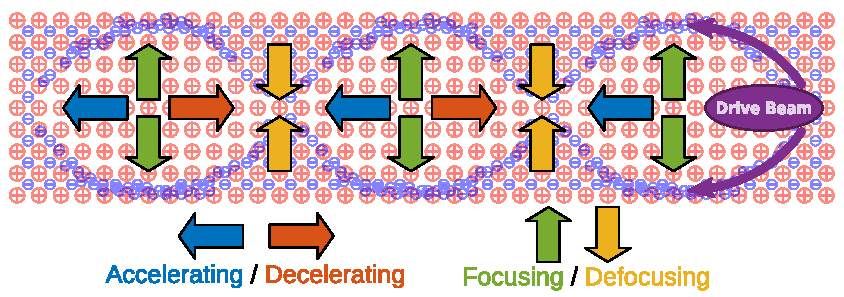
\includegraphics[width=0.85\linewidth,trim={0mm 0mm 0mm 0mm},clip]{figures/PlasmaWakefield}
    \caption{\label{Fig:PWFA:Illust} Illustration of a plasma wakefield accelerating structure with a single electron drive beam. A series of focusing/defocusing and accelerating/deceleratring regions (as seen for an electron witness beam) are produced behind the drive beam.}
\end{figure}

The principles behind beam driven plasma wakefield acceleration were formulated in the 1980s by Pisin Chen \emph{et al.} \cite{chen:1985}. The technique involves a beam of particles, called the \emph{drive beam}, travelling through a neutral plasma. The space charge of the drive beam displaces the plasma electrons, which oscillate at the plasma frequency, creating periodic regions of low and high electron density; see Eqs. (\ref{EQ:PWFA:L0W0}). The strong longitudinal and transverse electric fields generated by this wake is then loaded by a trailing beam of particles, called the \emph{witness beam}, which draws energy from the field in order to accelerate. We thus see a transfer of energy from the drive beam to the witness beam through plasma as the intermediate medium \cite{muggli:2009}.

The electrons displaced by the drive beam's space charge are pulled back on axis by the ions within the characteristic time $\omega_{p}^{-1}$. A conceptual illustration of an electron beam driven plasma accelerator is shown in Fig. \ref{Fig:PWFA:Illust}. Several regions of decreasing magnitude of accelerating/decelerating and focusing/defocusing are generated behind the drive beam. By positioning a trailing beam in an optimal phase, such a beam can both accelerated and focused. The drive beam needs to be shorter than the plasma period for this structure to develop, but multiple short drive beams with a separation of the plasma wave length can amplify the wakefields.

It has been shown experimentally that energy can be transferred from one or more electron drive beams to a single electron witness beam \cite{rosenzweig:1988, blumenfeld:2007, kallos:2008, litos:2014}. A limitation using an electron beams with a similar initial charge and energy for both drive and witness beams is that the witness beam will rapidly gain energy, while the drive beam loses energy. This causes the witness beam to catch up with the drive beam, so to speak, and the acceleration will therefore stop. Typically after a few tens of centimetres of plasma.

% ================================================================================================ %
\subsection{The Linear Regime}
\label{Int:PWFA:Lin}

A point like charge travelling at a speed close to the speed of light, will generate fields in its wake \cite{van_der_meer:1985, chen:1985}:
\begin{align}
    E_{z} &= -\frac{Q_{b}k_{pe}^{2}}{2\pi\epsilon_{0}} K_{0}(k_{pe}r)\cos(k_{pe}z - \omega_{pe}t) \label{EQ:PWFA:EZ} \\
    E_{r} &= \hphantom{-} \frac{Q_{b}k_{pe}^{2}}{2\pi\epsilon_{0}} K_{1}(k_{pe}r)\sin(k_{pe}z - \omega_{pe}t), \label{EQ:PWFA:ER}
\end{align}
where $Q_{b}$ is the charge of the beam, $k_{pe}$ is the plasma wave number, and $K_{0}$ and $K_{1}$ are modified Bessel functions. 

Cite \cite{ruth:1985}

% ================================================================================================ %
\subsection{The Non-Linear Regime}
\label{Int:PWFA:NLin}

Text

% ================================================================================================ %
\section{Protons vs. Electrons as Drive Beam}
\label{Int:PDPWFA}

Further details on proton driven plasma wakefield goes here.

Benefit of larger energy per bunch, challenge of producing short bunches.

Cite \cite{adli:2016a}.

% ================================================================================================ %
\section{The Self-modulation Instability}
\label{Int:SMI}

A long beam with respect to the plasma wavelength will generate a density wave driven by its own head. This is true for both laser beams \cite{esarey:1994} and particle beams \cite{kumar:2010}, and they are caused by the same underlying physics. For a laser beam, this produces alternating regions of focusing and diffraction. For a particle beam, the wakefields generated within the beam acts back on itself, breaking it up into short micro bunches with a surrounding, defocused halo.

In the 1980s, this self-modulating effect was taken advantage of in LWFA experiments as only long laser pulses were available. Advances in ultra short laser technology later removed the dependence of this effect \cite{pukhov:2002}, however for proton drive beams this is still an issue. For instance, the SPS proton beam used by AWAKE is orders of magnitude longer than the plasma wavelength needed for the experiment.

The self-modulation instability (SMI), is one of several instabilities affecting long beams in plasma.

% To add: Phase velocity of SMI WF. Two-stream and hosing.

In electron beam \cite{muggli:2014}.

% ================================================================================================ %
\section{Numerical Simulations of PWFA}
\label{Int:Sim}

PIC codes. Osiris vs, QuickPIC.

Numerical Cherenkov, Lehe. Relevance to emittance.

Reference to PIC appendix.

Maybe something about resolution and convergence.

% ================================================================================================ %
